\documentclass[tikz,border=6pt]{standalone}
\usepackage{tikz}
\usepackage{xcolor}

\definecolor{detectblue}{RGB}{51,108,229}
\definecolor{recoveryorange}{RGB}{239,108,0}
\definecolor{imperativegray}{RGB}{102,102,102}

\begin{document}
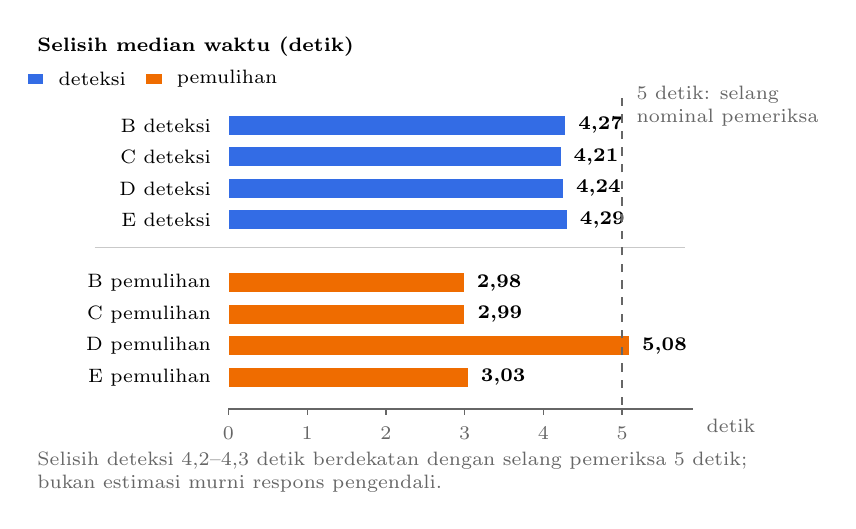
\begin{tikzpicture}[
    x=1cm, y=1cm,
    bar/.style={draw=none, fill=#1, inner sep=0pt},
    label/.style={font=\scriptsize, anchor=east},
    value/.style={font=\scriptsize\bfseries, anchor=west}
]

% Legend and title
\node[font=\scriptsize\bfseries, anchor=west] at (-2.55,7.55) {Selisih median waktu (detik)};
\fill[detectblue] (-2.55,7.08) rectangle (-2.35,7.20);
\node[font=\scriptsize, anchor=west] at (-2.28,7.14) {deteksi};
\fill[recoveryorange] (-1.05,7.08) rectangle (-0.85,7.20);
\node[font=\scriptsize, anchor=west] at (-0.78,7.14) {pemulihan};

% Detection bars
\node[label] at (-0.10,6.55) {B deteksi};
\node[bar=detectblue, minimum width=4.27cm, minimum height=0.24cm, anchor=west] at (0,6.55) {};
\node[value] at (4.32,6.55) {4,27};

\node[label] at (-0.10,6.15) {C deteksi};
\node[bar=detectblue, minimum width=4.21cm, minimum height=0.24cm, anchor=west] at (0,6.15) {};
\node[value] at (4.26,6.15) {4,21};

\node[label] at (-0.10,5.75) {D deteksi};
\node[bar=detectblue, minimum width=4.24cm, minimum height=0.24cm, anchor=west] at (0,5.75) {};
\node[value] at (4.29,5.75) {4,24};

\node[label] at (-0.10,5.35) {E deteksi};
\node[bar=detectblue, minimum width=4.29cm, minimum height=0.24cm, anchor=west] at (0,5.35) {};
\node[value] at (4.34,5.35) {4,29};

% Separator
\draw[imperativegray!35, line width=0.5pt] (-1.7,5.00) -- (5.8,5.00);

% Recovery bars
\node[label] at (-0.10,4.55) {B pemulihan};
\node[bar=recoveryorange, minimum width=2.98cm, minimum height=0.24cm, anchor=west] at (0,4.55) {};
\node[value] at (3.03,4.55) {2,98};

\node[label] at (-0.10,4.15) {C pemulihan};
\node[bar=recoveryorange, minimum width=2.99cm, minimum height=0.24cm, anchor=west] at (0,4.15) {};
\node[value] at (3.04,4.15) {2,99};

\node[label] at (-0.10,3.75) {D pemulihan};
\node[bar=recoveryorange, minimum width=5.08cm, minimum height=0.24cm, anchor=west] at (0,3.75) {};
\node[value] at (5.13,3.75) {5,08};

\node[label] at (-0.10,3.35) {E pemulihan};
\node[bar=recoveryorange, minimum width=3.03cm, minimum height=0.24cm, anchor=west] at (0,3.35) {};
\node[value] at (3.08,3.35) {3,03};

% Axis
\draw[imperativegray, line width=0.7pt] (0,2.95) -- (5.9,2.95);
\foreach \x in {0,1,2,3,4,5} {
    \draw[imperativegray, line width=0.5pt] (\x,2.95) -- (\x,2.87);
    \node[font=\scriptsize, text=imperativegray, anchor=north] at (\x,2.84) {\x};
}
\node[font=\scriptsize, text=imperativegray, anchor=north west] at (5.95,2.95) {detik};

% Reference line
\draw[imperativegray, dashed, line width=0.8pt] (5.0,3.00) -- (5.0,6.90);
\node[font=\scriptsize, text=imperativegray, anchor=south west, align=left] at (5.06,6.42)
    {5 detik: selang\\nominal pemeriksa};
\node[font=\scriptsize, text=imperativegray, anchor=north west, align=left] at (-2.55,2.52)
    {Selisih deteksi 4,2--4,3 detik berdekatan dengan selang pemeriksa 5 detik;\\bukan estimasi murni respons pengendali.};

\end{tikzpicture}
\end{document}
